\chapter{Procesos}
\begin{BPMN}{PROC-01}{Creación de un Programa Académico}{}
    \PCitem{Participantes}{Unidad Académica, DES, Consejo General Consultivo y Direccion General}
    \PCitem{Objetivo}{La elaboración o renovación de los Programas Académicos  del IPN, partiendo desde el análisis de la propuesta, la elaboración del plan de estudios hasta la conformación del mapa curricular y las unidades de aprendizaje, siendo revisado en cada etapa por las autoridades correspondientes}
    \PCitem{Interrelación con otros procesos}{}
    \PCitem{Proveedores}{Agentes internos o externos del IPN}
    \PCitem{Entradas}{Propuesta de creación o renovación de programa académico}
    \PCitem{Consumidores}{Unidad Académica, DES, Consejo General Consultivo y Direccion General}
    \PCitem{Salidas}{Programa académico}
    \PCitem{Precondiciones}{Solicitud de nuevo programa académico}
    \PCitem{Postcondiciones}{Aplicacion del nuevo programa academico}
    \PCitem{Frecuencia}{}
    \PCitem{Tipo}{Operativo}
    \PCitem{Áreas de oportunidad}{Registro y revisión de planes de estudio, mapas curriculares y unidades de aprendizaje en línea }
\end{BPMN}
En la figura \hyperref[]{}
\begin{figure}[htbp]
	\begin{center}
		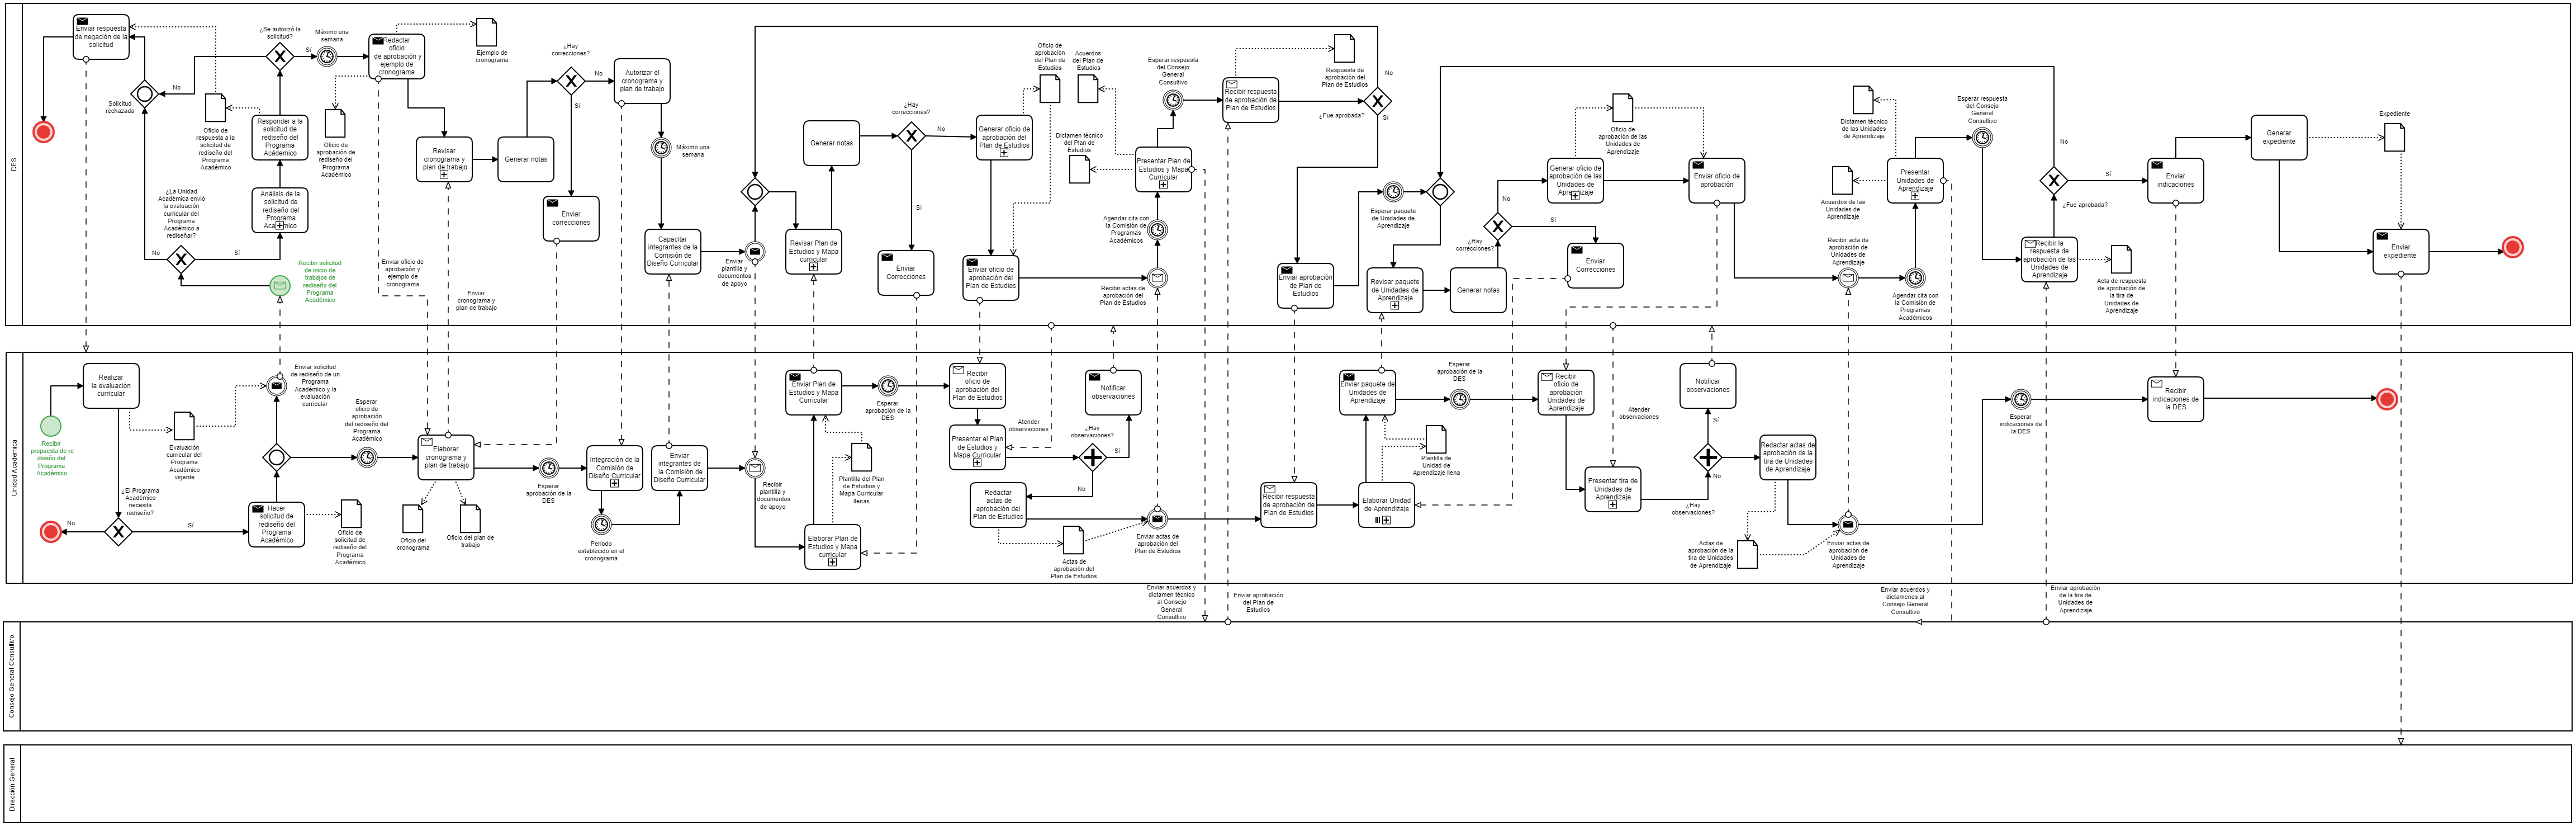
\includegraphics[width=.95\textwidth]{C1-DP/MP/bpmnMacro.png}
		\caption{}
		\label{fig:}
	\end{center}
\end{figure}
\section{Descripción}
\begin{itemize}
	\item \textbf{Elaborar plan de estudios y mapa curricular:} En la unidad académica en el jefe de innovación educativa asigna un docente para que elabore el plan de estudios y mapa curricular de programa académico llenado las plantillas o realice las correcciones de los documentos con notas recibidos de la DES.  
	\item \textbf{Enviar plan de estudios y mapa curricular:} Al terminar la elaboración de plan de estudios y el mapa curricular la unidad académica envía por correo electrónico los documentos de los respectivos archivos a la DES en especifico a la división de innovación académica.  
	\item \textbf{Revisar plan de estudios y mapa curricular:} El jefe del departamento de desarrollo e innovación curricular recibe los documentos y asigna al personal (analistas) encargados de revisar los documentos o puede hacerlo el mismo. 
	\item \textbf{Generar notas:} El encargado de la revisión leerá el documento e ira subrayando y agregando notas en todas las secciones que considere necesario debido a que presentan errores de estructura, coherencia u ortografía.   
	\item \textbf{Enviar correcciones plan de estudios y mapa curricular:}Al terminar la revisión el jefe del departamento de desarrollo e innovación curricular envía los documentos con las respectivas notas de regreso a la unidad de académica por correo electrónico, todo este caso de que se hayan generado notas. 
	\item \textbf{Generar oficio de aprobación del  plan de estudios:}---------
	\item \textbf{Enviar oficio de aprobación del plan de estudios:}-----------
	\item \textbf{Recibir oficio de aprobación del plan de estudios:}----------
	\item \textbf{Presentar el plan de estudios y mapa curricular:}------------
	\item \textbf{Presentar el plan de estudios y mapa curricular DES:}--------
	\item \textbf{Redactar actas de aprobación del plan de estudios:}----------
	\item \textbf{Recibir respuesta de aprobación del plan de estudios:}-------
	\item \textbf{Enviar aprobación de plan de estudios:}---------------
	\item \textbf{Recibir aprobación del plan de estudios:}-------------
	\item \textbf{Elaborar unidad de aprendizaje:} En la unidad académica el jefe de innovación educativa, asigna el docente encargado de llenar la plantilla de la información de un unidad de aprendizaje, esto lo debe hacer con un conjunto de unidades de aprendizaje con el propósito de juntar un semestre como mínimo o realice las correcciones de los documentos con notas recibidos de la DES .     
	\item \textbf{Enviar paquete de  unidades de aprendizaje:} El jefe de innovacion educativa  envía por correo electrónico los documentos que comprenden el paquete de unidades de aprendizaje  
	\item \textbf{Revisar paquete de  unidades de aprendizaje:}El jefe del departamento de desarrollo e innovación curricular recibe los documentos y asigna al personal (analistas) encargados de revisar los documentos repartiéndolos por unidad de aprendizaje, el se puede asignar uno también . 
	\item \textbf{Generar notas de  unidades de aprendizaje:} El encargado de la revisión leerá el documento e ira subrayando y agregando notas en todas las secciones que considere necesario debido a que presentan errores de estructura, coherencia u ortografía.  
	\item \textbf{Enviar correcciones unidades de aprendizaje:} Al terminar la revisión el jefe del departamento de desarrollo e innovación curricular envía los documentos con las respectivas notas de regreso a la unidad de académica por correo electrónico, todo este caso de que se hayan generado notas. 
	
\end{itemize}